% Section 3, Problem Setup and Metrics.
\section{Problem Setup and Metrics}
\label{sec:problem}

\subsection{Task and Cost Model}
\label{sec:problem:task}

We study repo-level issue resolution: given the text of an issue and a
snapshot of the repository, the system must produce a source-code patch
whose correctness is judged by held-out tests~\citep{swebench,swebenchpro}.
Frontier language models already solve these tasks at high rates, but their
per-task cost is substantial.  Strong open-weights models are far cheaper
yet less reliable.  In a deployment that selects from a pool of candidate
\emph{fixer} models, the natural question is whether one can retain the
strongest model's effectiveness while spending less.

To answer that question we adopt a single yardstick, defined before any
experiment: \textbf{total cost per solve at a matched solve rate}.
``Total'' means every system component's spend, including searcher GPU
time, verification sandboxes, and fixer API calls, not just the final
model invocation.  A system claims a cost improvement only if its solve
rate matches that of the best individual model.

This metric exposes a trivial lower bound.  Any point on the line segment
between a cheap model's (cost, accuracy) and a strong model's (cost,
accuracy) is achievable by randomly splitting traffic between the two, a
strategy we call \emph{blind mixing}.  A routing system is interesting
only if it operates above that segment.  We describe the operational
details of the blind-mixing line in~\S\ref{sec:setup}.

\subsection{Why Accuracy-Only Routing Is Insufficient}
\label{sec:problem:audit}

Before building \sysname we replayed a set of learned routers over the
publicly available per-task results of three SWE-coding benchmarks:
SWE-bench Verified~\citep{swebenchverified}, SWE-bench
Multilingual~\citep{swebenchmultilingual}, and SWE-bench
Pro~\citep{swebenchpro}.  The replay incurs zero model cost, and the
routers span four families: embedding retrieval ($k$-NN), trained heads
(logistic and MLP), clustering, and a language-rule baseline.  Two
findings shaped the design that followed.

First, solve sets are strongly nested: the tasks a weaker model solves
are largely a subset of those the strongest model solves.  Measured as set
containment, the overlap is 0.941, 0.912, and 0.773 across the three
benchmarks.  Nor is this an artifact of comparing cheap models with
frontier ones: replaying pools built from frontier models alone, one per
lab, leaves containment at 0.90 to 0.93.  These models are generally
strong rather than complementary specialists, so an accuracy-oriented
router has almost no room to combine their strengths.
Figure~\ref{fig:solve-sets} sketches the consequence: between any two
models the accuracy prize is only a thin sliver, while the large shared
region is where a cheaper model would have sufficed all along.

\begin{figure}[!tbp]
\centering
% ===========================================================================
% fig-solve-sets.tex — two stacked panels: (a) two frontier peers nearly
% coincide, so accuracy routing has no headroom; (b) a cheaper model's set
% sits mostly inside the strongest model's, which is where cost routing pays.
% BODY ONLY (tikzpicture in a \resizebox). Wrapper/caption/label live in the
% section file; mounts as a single-column \begin{figure}[!tbp].
% Requires % ===========================================================================
% fig-style.tex — shared colour / marker scheme for EVERY main-paper figure.
% \input this ONCE from the preamble of main.tex (after tikz + pgfplots).
%
% House rule: the palette is defined here and nowhere else. Each series also
% gets a distinct marker AND line style so the figures survive grayscale
% printing.
%
%   \sysname / deployed .. cSys   (blue!70!black)    mark *
%   opus / claude ........ cOpus  (red!70!black)     mark square*
%   gpt .................. cGpt   (teal!70!black)    mark triangle*
%   kimi ................. cKimi  (violet!70!black)  mark diamond*
%   flash ................ cFlash (orange!70!black)  mark pentagon*
%   greedy / baseline .... cBase  (gray)             mark o
% ===========================================================================
% The pipeline diagram needs the calc library for coordinate arithmetic; the
% rest of the libraries are already loaded in main.tex's preamble.
\usetikzlibrary{calc}
% Hatching, so bar charts stay readable in grayscale.
\usetikzlibrary{patterns}

\colorlet{cSys}{blue!70!black}
\colorlet{cOpus}{red!70!black}
\colorlet{cGpt}{teal!70!black}
\colorlet{cKimi}{violet!70!black}
\colorlet{cFlash}{orange!70!black}
\colorlet{cBase}{gray}

% Common axis furniture: footnotesize ticks/legend, small titles, framed
% legend in gray!50, light horizontal grid.
\pgfplotsset{
  paperaxis/.style={
    width=0.80\linewidth,
    height=5.2cm,
    tick label style={font=\footnotesize},
    label style={font=\footnotesize},
    title style={font=\small},
    legend style={font=\footnotesize, draw=gray!50, fill=white,
                  fill opacity=0.9, text opacity=1, rounded corners=1pt},
    every axis plot/.append style={line width=0.7pt},
    grid style={gray!25, line width=0.3pt},
    axis line style={gray!60},
    tick style={gray!60},
  },
  papermark/.style={mark size=2.6pt},
}
 in the preamble.
%
% PROVENANCE
%   Schematic, illustrative only, no measured quantities. Blob sizes, the
%   crescent widths and the sliver width are drawn for legibility, not to
%   scale; the figure carries no numbers and names no benchmark or model.
%   The qualitative claims it illustrates (frontier peers' solve sets nearly
%   coincide; a weaker model's solve set is largely contained in the
%   strongest model's) are stated with their measured containment values in
%   the body text of \S\ref{sec:problem:audit} and Appendix~\ref{apx:audit}.
%
%   Colour contract (fig-style.tex): the sets themselves are neutral cBase
%   grays, since no blob is a component we build; the cSys tint marks only
%   the region the paper acts on (route the shared region for cost). Both
%   panels share one lightness ladder, so the nesting and the rarity of the
%   exclusive regions survive grayscale printing:
%   white (neither) < cBase!12 (shared) < cSys!13 (shared, acted on)
%   < cBase!36 (solved by only one model).
%
% GEOMETRY NOTE
%   Panel (a): two equal ellipses, radii (1.90, 0.86), centres 0.46 apart,
%   so about 85% of each area is shared. The exclusive crescents are drawn
%   wider than their true relative size, otherwise the pair reads as a
%   single ring at print scale.
%   Panel (b): the cheap set pokes outside the strong set only over
%   x = 5.84 .. 6.06, a ~2mm sliver.
%
% LAYOUT NOTE
%   Per-panel dashed universe boxes beat one box around both panels: a
%   shared box left the two ellipse groups floating in a tall empty frame,
%   and the panel kickers had nowhere to sit that did not read as a caption
%   for the whole frame. "all tasks" names the box once, in panel (a).
% ===========================================================================
\resizebox{\linewidth}{!}{%
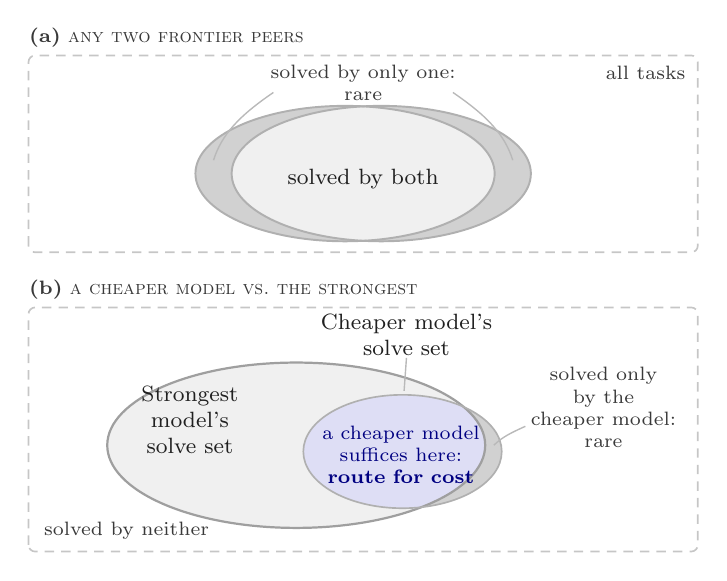
\begin{tikzpicture}[
  x=1cm, y=1cm,
  lbl/.style={font=\footnotesize, text=gray!25!black, align=center,
              inner sep=0pt},
  micro/.style={font=\scriptsize, text=gray!45!black, align=center,
                inner sep=0pt},
  kick/.style={font=\scriptsize\scshape, text=gray!45!black, inner sep=0pt},
  lead/.style={gray!55, line width=0.5pt},
  uni/.style={gray!45, line width=0.6pt, rounded corners=2.4pt,
              dash pattern=on 1.2mm off 0.9mm},
]

% =========================================================================
% PANEL (a) — any two frontier peers
% =========================================================================
\draw[uni] (0.05,3.85) rectangle (8.55,6.35);
\node[kick, anchor=south west] at (0.05,6.45)
  {{\upshape\bfseries (a)}~any two frontier peers};
\node[micro, anchor=north east] at (8.40,6.22) {all tasks};

\def\PA{(4.07,4.85)} \def\PB{(4.53,4.85)} \def\PR{(1.90 and 0.86)}

\fill[cBase!36] \PA ellipse \PR;
\fill[cBase!36] \PB ellipse \PR;
\begin{scope}
  \clip \PA ellipse \PR;
  \fill[cBase!12] \PB ellipse \PR;
\end{scope}
\draw[gray!62, line width=0.7pt] \PA ellipse \PR;
\draw[gray!62, line width=0.7pt] \PB ellipse \PR;

\node[lbl] at (4.30,4.78) {solved by both};

% one shared callout for the two thin crescents
\node[micro, text width=2.6cm] at (4.30,6.00)
  {solved by only one:\\rare};
\draw[lead] (3.16,5.88) .. controls (2.72,5.58) and (2.50,5.34) .. (2.40,5.02);
\draw[lead] (5.44,5.88) .. controls (5.88,5.58) and (6.10,5.34) .. (6.20,5.02);

% =========================================================================
% PANEL (b) — a cheaper model vs the strongest
% =========================================================================
\draw[uni] (0.05,0.05) rectangle (8.55,3.15);
\node[kick, anchor=south west] at (0.05,3.25)
  {{\upshape\bfseries (b)}~a cheaper model vs.\ the strongest};

\def\SC{(3.45,1.40)} \def\SR{(2.40 and 1.05)}
\def\CC{(4.80,1.32)} \def\CR{(1.26 and 0.72)}

% 1. cheap set underneath — what stays visible is the sliver outside
\fill[cBase!36] \CC ellipse \CR;
% 2. strong set on top — covers everything it contains
\fill[cBase!12] \SC ellipse \SR;
% 3. the intersection, the region this paper acts on
\begin{scope}
  \clip \SC ellipse \SR;
  \fill[cSys!13] \CC ellipse \CR;
\end{scope}

\draw[cBase!75, line width=0.8pt] \SC ellipse \SR;
\draw[gray!62, line width=0.6pt]  \CC ellipse \CR;

\node[lbl, text width=2.0cm] at (2.10,1.72)
  {Strongest model's\\solve set};

\node[lbl, text width=2.2cm] at (4.85,2.80)
  {Cheaper model's\\solve set};
\draw[lead] (4.85,2.51) -- (4.82,2.09);

\node[micro, text=cSys!72!black, text width=2.1cm] at (4.78,1.28)
  {a cheaper model\\suffices here:\\\textbf{route for cost}};

\node[micro, anchor=west, text width=1.85cm] at (6.42,1.88)
  {solved only by the\\cheaper model:\\rare};
\draw[lead] (6.36,1.64) .. controls (6.18,1.56) and (6.06,1.50) .. (5.96,1.40);

\node[micro, anchor=west] at (0.24,0.32) {solved by neither};

\end{tikzpicture}}

\caption{\textbf{Solve sets are nearly nested (schematic).} (a)~Even two
frontier peers solve almost the same tasks, so accuracy routing has little
to win. (b)~A cheaper model's set sits mostly inside the strongest
model's; that shared region is where routing for cost pays.}
\label{fig:solve-sets}
\end{figure}

Second, no learned router we tested exceeded the solve rate of
always picking the strongest model; every observed gap fell within noise.
Taken together, these results suggest a plain conclusion: routing for
\emph{accuracy} has little headroom on current issue-resolution
benchmarks.  Routing for \emph{cost}, by contrast, does not require
complementary skills at all.  It requires only the ability to predict when
a cheaper model will suffice.  Full audit tables appear in Appendix~\ref{apx:audit}.

\subsection{Goal}
\label{sec:problem:goal}

Our objective inverts the premise of prior routing work.  Rather than
seeking accuracy gains by combining models, we aim to match the strongest
available model's solve rate at a materially lower total cost per solve.

The thesis is that routing should happen \emph{after} engaging with the
problem, not from the task text alone.  In \sysname a small searcher
model first explores the repository; both its explicit work product (a
structured handoff) and its internal representation of the task (hidden
states) then inform the routing decision.
The evaluation partly supports this thesis: the engagement's payoff
arrives through the handoff more than through the routing decision
(\S\ref{sec:results}).
\S\ref{sec:system} details the architecture.
